\documentclass{standalone}
\usepackage{tikz}
\usepackage{ctex,siunitx}
\setCJKmainfont{Noto Serif CJK SC}
\usepackage{tkz-euclide}
\usepackage{amsmath}
\usetikzlibrary{patterns, calc,3d}
\usetikzlibrary {decorations.pathmorphing,decorations.pathreplacing,decorations.shapes}
\tikzset{label style/.append style={font=\small}}
\begin{document}
\small
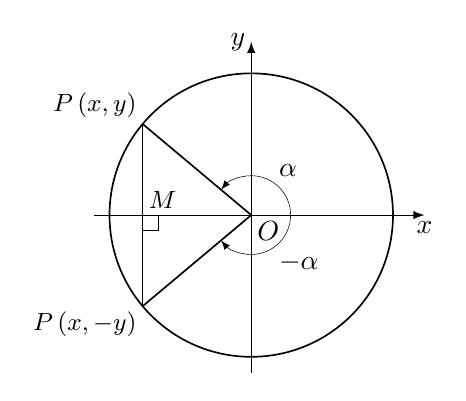
\begin{tikzpicture}[>=latex,scale=1.0,inner sep=2pt]
  \tkzDefPoint(220:1.8){N'}
  \tkzDefPoint(140:1.8){M'}
  \tkzDefPoints{0/0/O,2/0/x}
  \tkzDefPointsBy[projection=onto O--x](M'){M};
  \draw[->](-2,0)--(2.2,0)node[below]{$x$};
  \draw[->](0,-2)--(0,2.2)node[left]{$y$};
  \node at (0,0)[below right]{$O$};
  \draw[semithick](0,0)circle(1.8)(O)--(N')(O)--(M');
  \draw[very thin,->](0.5,0)arc(0:140:0.5)node[pos=0.4,above right]{$\alpha$};
  \draw[very thin,->](0.5,0)arc(0:-140:0.5)node[pos=0.4,below right]{$-\alpha$};
  \tkzLabelPoints[above right](M)
  \tkzLabelPoint[above left](M'){$P\,(x,y)$}
  \tkzLabelPoint[below left](N'){$P\,(x,-y)$}
  \tkzMarkRightAngle[size=0.2](N',M,O)
  \tkzDrawSegments(N',M')
\end{tikzpicture}
\end{document}